\section{Đặt vấn đề}
Sau sự thành công của DeepMind năm 2013 với bộ máy chơi game đình đám một thời Atari\cite{DBLP:journals/corr/MnihKSGAWR13}, \word{Học Tăng cường}{Reinforcement Learning}đã bước vào các ngành công nghiệp trò chơi điện tử nhằm đạt giải quyết được những bài toán phức tạp và tạo nên những thử thách mới cho con người. Đây là bước ngoặt quan trọng cho sự trở lại mãnh liệt sau khoảng thời gian lặng tiếng của phương pháp học tăng cường khi AlphaGo\cite{44806} đánh bại kỳ thủ xuất xắc nhất lúc bấy giờ trong bộ môn cờ vây năm 2017. Tiếp sau đó là sự thành công của OpenAI trong trò chơi Dota2\cite{openai2019dota} , những người chơi được đánh giá mạnh nhất của trò chơi vào thời điểm này "ngả mũ" trước những nhân vật được máy điều khiển . Với bảng thành tích như vậy, học tăng cường thực sự giải quyết được những vấn đề mà con người khó có thể đạt được tuy nhiên việc áp dụng học tăng cường vào thực tế rất khó khăn theo như\cite{DBLP:journals/corr/abs-1904-12901}.\\
\\
The World’s Hardest Game\cite{WHGwebsite} (WHG) là một trò chơi trực tuyến nổi tiếng trong năm 2015 với vòng chơi khó nhưng đủ khiến kích thích người chơi cố gắng vượt qua bởi tưởng “dễ nhưng không dễ” của nó. Trong trò chơi, người chơi có thể di chuyển bằng 5 hướng (trên, dưới, trái, phải, đứng yên) với mục đích hoàn thành cách thức chơi của mỗi vòng. Để hoàn thành một vòng chơi, người chơi phải thu thập hết các đồng xu, tránh va phải các vật cản và di chuyển đến vùng qua màn. Vì các yếu tố của trò chơi thảo mãn \cite{MarkovProperty} và độ khó của trò chơi nên WHG là ứng cử viên tốt cho học tăng cường.\\
\begin{figure}[h]
    \centering
    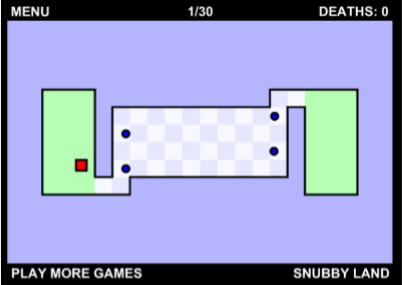
\includegraphics[height=0.3\textheight]{Pic/lv1game.png}
    \caption[Vòng đầu tiên của WHG]{\textit{Hình ảnh vòng đầu tiên của WHG}, trò chơi chia làm 3 phần: phần xanh lá cây trái cùng là vùng an toàn, phần xanh phải cùng là vùng đích chiến thắng và còn lại là vùng hoạt động của các vật cản. Trên hình, biểu tượng ô vuông màu đỏ biểu thị cho robot và biểu tượng tròn màu xanh biểu thị cho các vật cản chuyển động.}
    \label{fig:lv1game}
\end{figure}
\section{Mục tiêu}
Một vài các tiếp cận của học tăng cường vào WHG như sử dụng \word{Giải thuật Di truyền}{Genetic Algorithm}của \cite{WHG_codebullet} hay đưa ra các trò chơi nhỏ của \cite{WHG_yasyf}, cả hai cách tiếp cận trên đều không đưa ra được lời giải cho WHG nhưng đã để lại nhiều kinh nghiệm cho nhóm tác giả trong việc chinh phục WHG.\\
Mục tiêu chính của khóa luận này là thực hiện huấn luyện một \word{robot}{agent}\footnote{Nghĩa của agent ở đây nhóm tác giả chọn đại diện cho sự vật này là robot để thể hiện cho sự vật cần học các tri giác vì "tác tử" được dùng để gọi agent có thể khiến người đọc nhầm lẫn.} đủ thông minh để chinh phục WHG và đường đi tìm được phải tối ưu. Ngoài ra sau các thử nghiệm của \cite{WHG_yasyf} khi sử dụng \word{Học Tăng cường Chuyên sâu}{Deep Q-learning}vào WHG nhưng chưa kết quả không khả quan, vì vậy chúng tôi sẽ đưa ra các giải pháp để áp dụng học tăng cường vào WHG cùng với các tùy chỉnh sẽ đưa ra trong xuyên suốt khóa luận.\\
Kết quả và thực nghiệm sau cùng của nhóm sẽ được cập nhật tại:\\
\textbf{\href{https://github.com/pqkhanh561/thesis}{https://github.com/pqkhanh561/thesis}}

\section{Cấu trúc khóa luận}
Theo sau chương giới thiệu này, khóa luận sẽ bao quát lý thuyết học tăng cường và các thực nghiệm trên các môi trường đề xuất.
\begin{labeling}{alligator}
\item [\textbf{Chương 1:}] Phần giới thiệu đưa ra tổng quan về khóa luận, bao gồm các tiếp cận tới bài toán hiện tại, động lực để nhóm thực hiện và cuối cùng là mục tiêu của của nhóm tác giả hướng đến.
\item [\textbf{Chương 2:}] Đưa ra lý thuyết cơ bản của học tăng cường và sự hình thành Q-learning.
\item [\textbf{Chương 3:}] Bao quát các bước thực hiện khóa luận, bao gồm các cài đặt để có thể thực hiện huấn luyện và đưa ra một số giả thiết cùng các giải pháp cải thiện.
\item [\textbf{Chương 4:}] Trình bày các kết quả huấn luyện của các mô hình được đề xuất, thảo luận các bước đi tiếp theo sau những thay đổi trong quá trình.
\item [\textbf{Chương 5:}] Kết luận từ các kết quả của nhóm.
\item [\textbf{Chương 6:}] Nhóm tác giả đưa ra các hướng đi trong tương lai cho đề tài.
\end{labeling}
